% !TEX encoding = utf8
% !TeX spellcheck = pl_PL


\documentclass[a4paper, 10pt]{article}
\usepackage[utf8]{inputenc}
\usepackage[polish]{babel}
\usepackage{polski}
\usepackage{graphicx}
\usepackage{listings}
\usepackage{amsfonts}
\usepackage{amsmath}
\usepackage{geometry}

\usepackage{float}


\author{Jakub Postępski}
\title{STP - Projekt 2.24}
\graphicspath{{../images/}}
\newgeometry{tmargin=3cm, bmargin=0.5cm, lmargin=0.5cm, rmargin=0.5cm}

\begin{document}
	\maketitle
	\section{Wyznaczanie modeli rekurencyjnych}
	Dla podanych danych wyznaczono modele rekurencyjne (tab. \ref{tab:z1}). Na początku przebiegu modele wykazują mniejszy błąd wyjścia. Wizualne obserwacje wyjść modeli potwierdzdają obliczenia błędu. \\
	Wybrano najlepszy model dla $\tau=6$. \\
	Dla najlepszego modelu: $b_6 = -0.1854$, $b_7=-0.918$, $a_1=-1.0403$, $a_2=0.1135$.\\
	Mamy:
	\[y(k)+a_1y(k-1) + a_2y(k-2)=b_6u(k-6)+b_7u(k-7)\]
	Po zastosowaniu transformaty $Z$:
	\[(1+a_1z^{-1} + a_2z^{-2})Y(z)=(b_6z^{-6}+b_7z^{-7})U(z)\]
	Więc transmitancja:
	\[G(z)=\frac{Y(z)}{U(z)}=\frac{b_6z^{-6}+b_7z^{-7}}{1+a_1z^{-1} + a_2z^{-2}}=\frac{-0.1854z^{-6}-0.918z^{-7}}{1-1.0403z^{-1} + 0.1135z^{-2}}\]
	\begin{table}[H]
	\begin{tabular}{|c|c|c|c|c|c|c|}
	\hline 
	$\tau$ & $b_\tau$ & $b_{\tau+1}$ & $-a_1$ & $-a_2$ & $E$ & rys. \\ 
	\hline 
	 1 & -0.0082 & -0.0679 &  1.6619 & -0.6799
	  & 79.2282 & \\ 
	\hline 
	2 & 0.0027 & -0.1003
	  &  1.5901 & -0.6135 & 54.2224 & \\ 
	\hline 3 & -0.0014 & -0.1337 &  1.4685  & -0.5010 & 39.9572 & \\ 
	\hline 
	4 & -0.0568 & -0.1271 & 1.3107 & -0.3552
	  & 32.3080  &\\ 
	\hline 
 5 & -0.1188 & -0.1281 & 1.1146 &  -0.1763 & 20.9694 & \\ 
	\hline 
	6 & -0.1854  &  -0.0918 &  1.0403  & -0.1135 & 16.3988 & \\ 
	\hline 
	7 & -0.1575 & -0.0517  & 1.2836 & -0.3445  & 46.8691
	& \\ 
	\hline
	8 & -0.1146 & 0.0001  & 1.5764 & -0.6144 & 176.8823 & \\ 
	\hline 
	\end{tabular}
	\label{tab:z1}
	\caption{Porównanie modeli rekurencyjnych}
	\end{table}
	
	\begin{figure}[H]
	\centering
	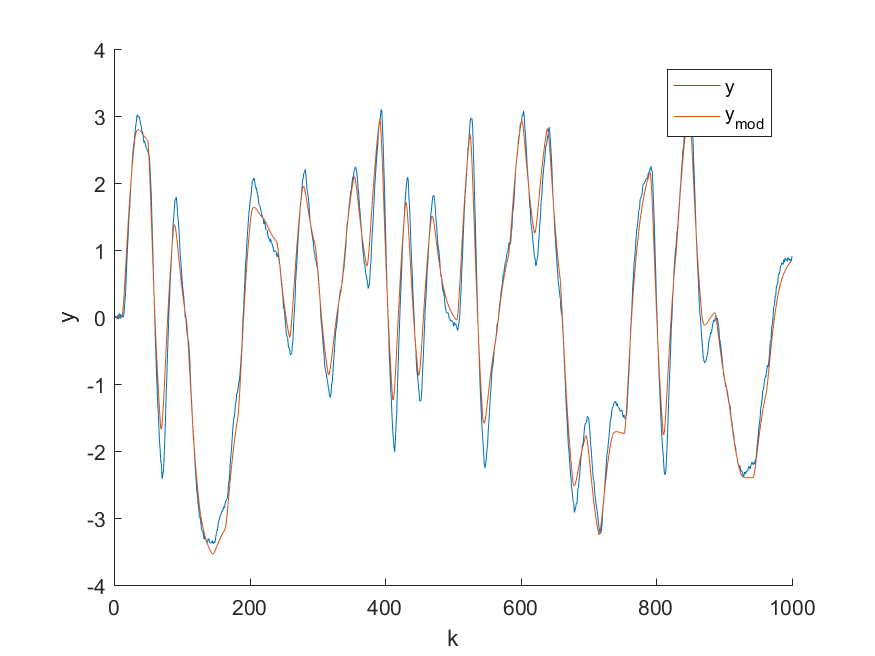
\includegraphics[width=0.9\linewidth]{z1_1}
	\caption{Wyjścia modelu dla $\tau=1$}
	\label{fig:z1_1}
	\end{figure}
	\begin{figure}[H]
	\centering
	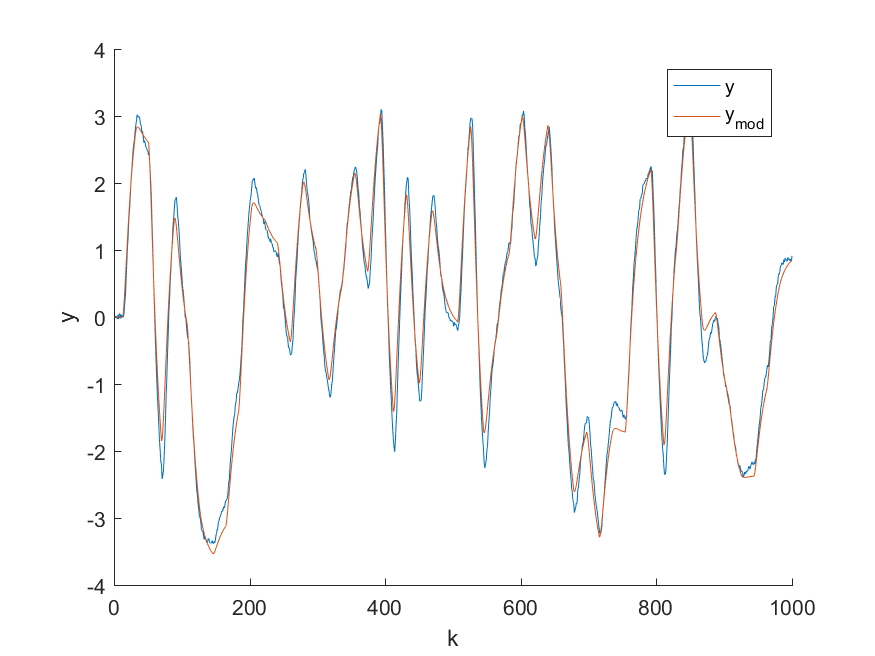
\includegraphics[width=0.9\linewidth]{z1_2}
	\caption{Wyjścia modelu dla $\tau=2$}
	\label{fig:z1_2}
	\end{figure}
	\begin{figure}[H]
	\centering
	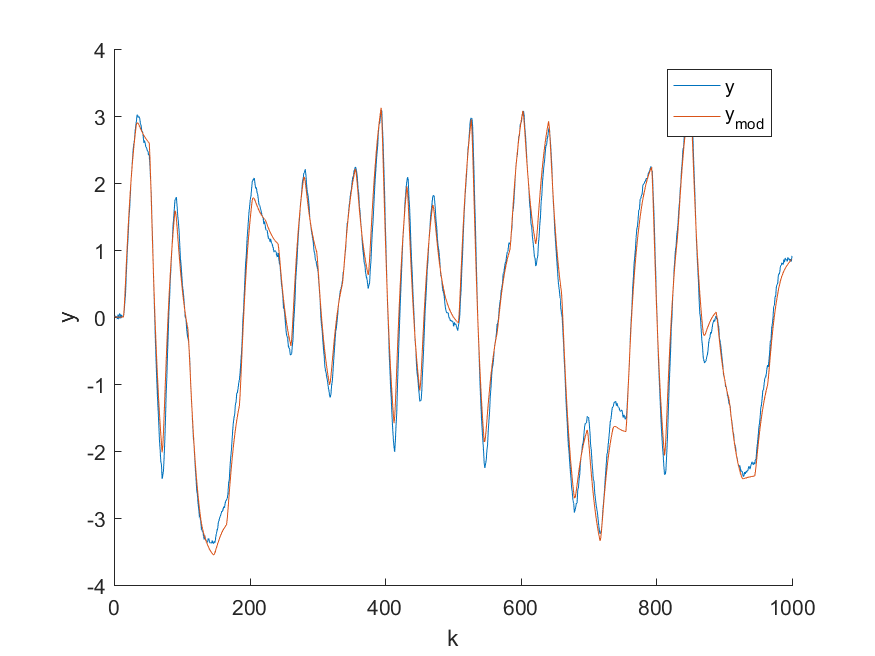
\includegraphics[width=0.9\linewidth]{z1_3}
	\caption{Wyjścia modelu dla $\tau=3$}
	\label{fig:z1_3}
	\end{figure}
	\begin{figure}[H]
	\centering
	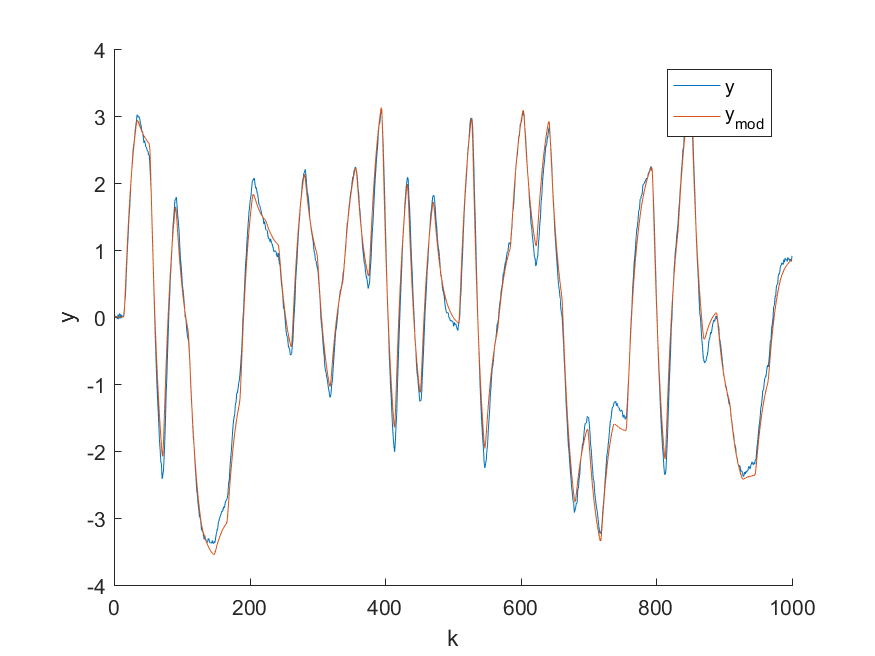
\includegraphics[width=0.9\linewidth]{z1_4}
	\caption{Wyjścia modelu dla $\tau=4$}
	\label{fig:z1_4}
	\end{figure}
	\begin{figure}[H]
	\centering
	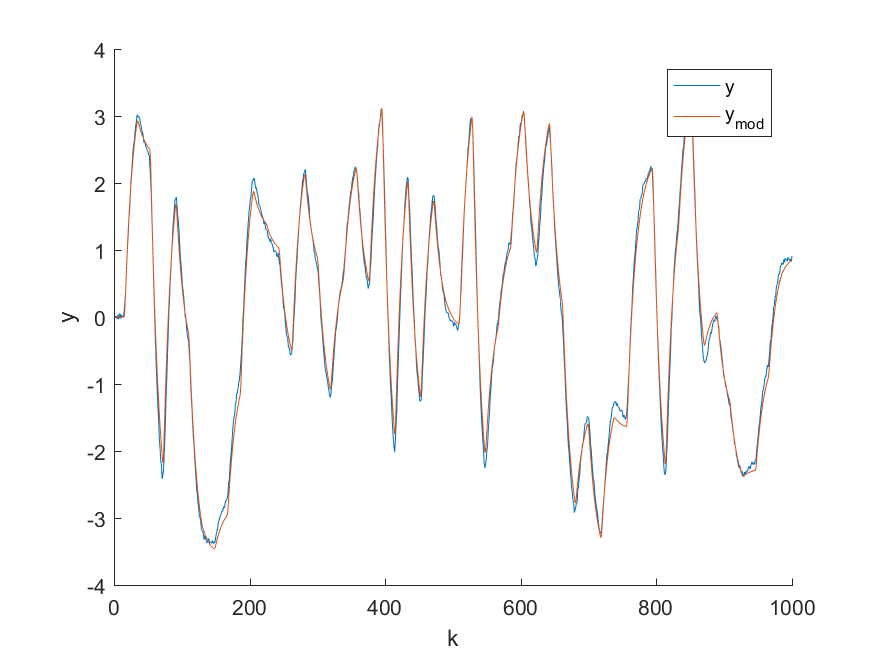
\includegraphics[width=0.9\linewidth]{z1_5}
	\caption{Wyjścia modelu dla $\tau=5$}
	\label{fig:z1_5}
	\end{figure}
	\begin{figure}[H]
	\centering
	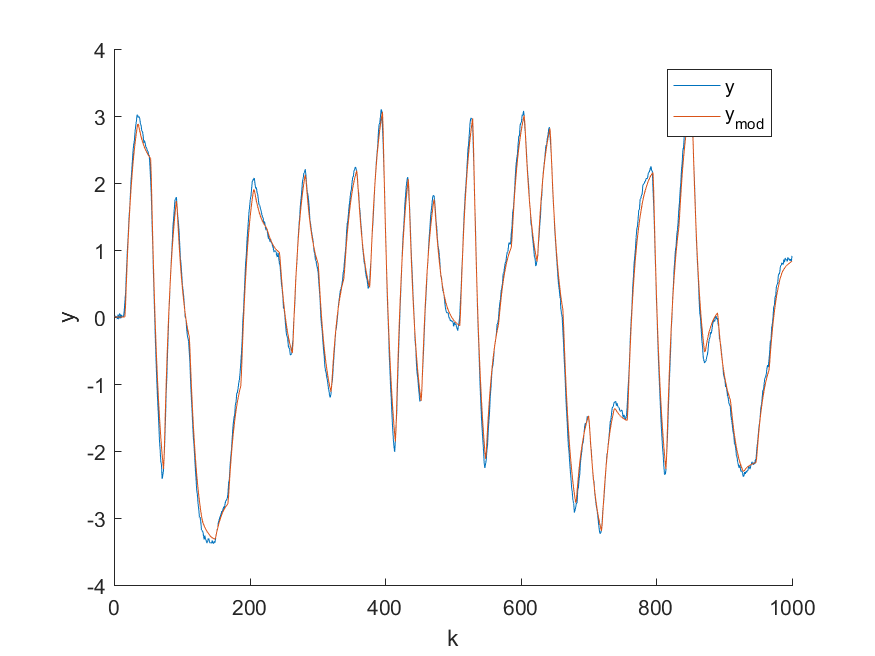
\includegraphics[width=0.9\linewidth]{z1_6}
	\caption{Wyjścia modelu dla $\tau=6$}
	\label{fig:z1_6}
	\end{figure}
	\begin{figure}[H]
	\centering
	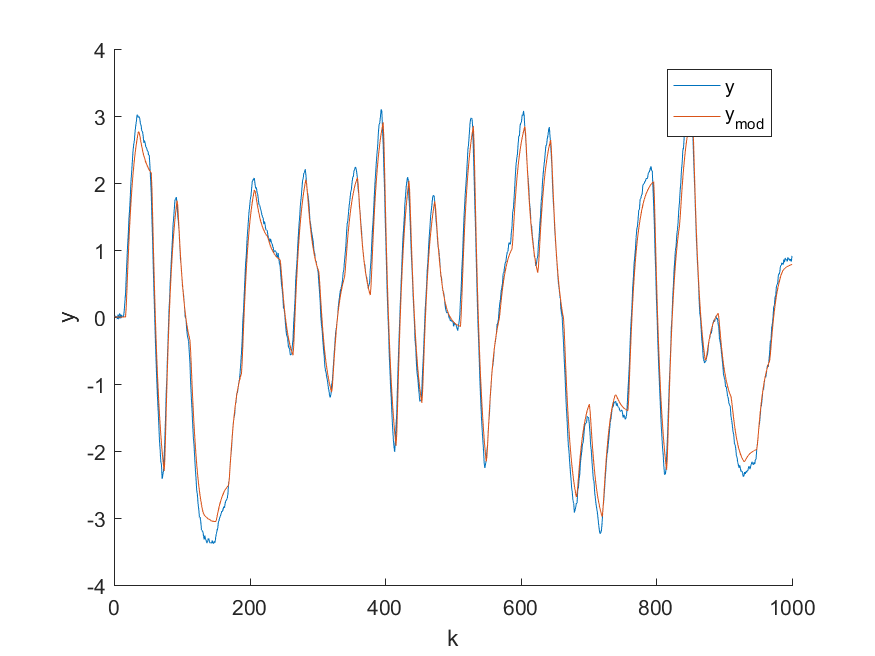
\includegraphics[width=0.9\linewidth]{z1_7}
	\caption{Wyjścia modelu dla $\tau=7$}
	\label{fig:z1_7}
	\end{figure}
	\begin{figure}[H]
	\centering
	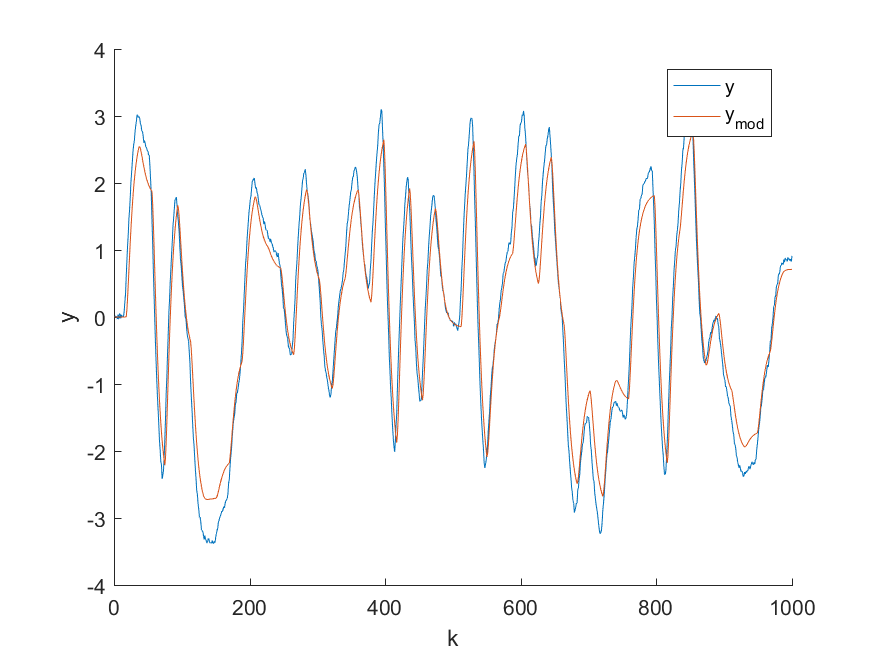
\includegraphics[width=0.9\linewidth]{z1_8}
	\caption{Wyjścia modelu dla $\tau=8$}
	\label{fig:z1_8}
	\end{figure}

	\section{Odpowiedz skokowa}
	Obliczono ze wzoru odpowiedz skokową (rys. \ref{fig:z2}).\\
	Wzmocnienie statyczne:
	\[K_{stat}=\lim_{z\rightarrow 1}G(z)=-3.7848\]
	\begin{figure}[H]
		\centering
		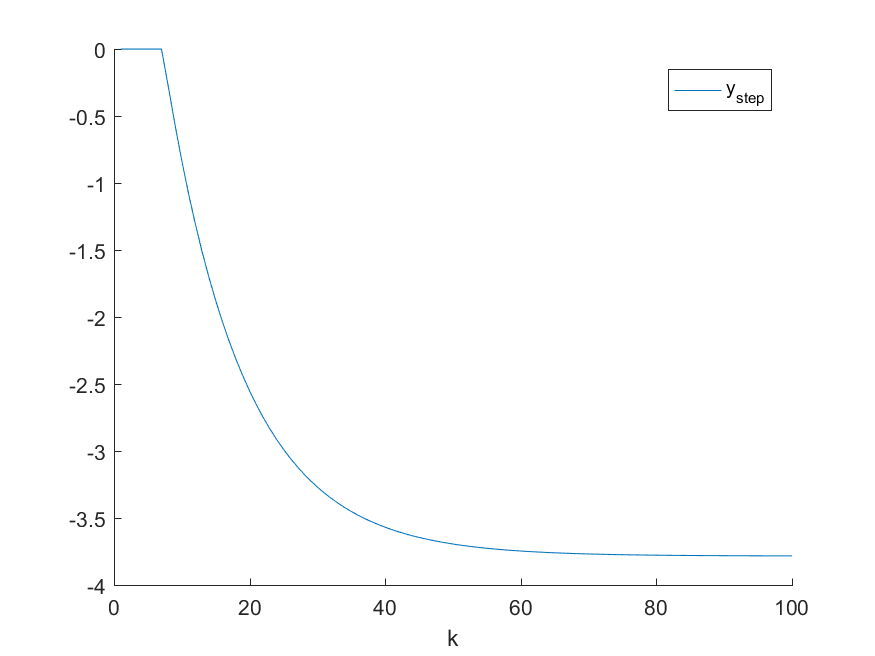
\includegraphics[width=0.9\linewidth]{z2}
		\caption{Odpowiedz skokowa modelu}
		\label{fig:z2}
		\end{figure}
\end{document}